
\section{Анализ предметной области}
\subsection{Задача классификации текстов}
Классификация текста —-- это процесс присвоения предопределенной категории или метки предложениям, абзацам, текстовым отчетам или неструктурированного текста.

За последние несколько десятилетий проблемы классификации текста широко изучались и решались во многих практических приложениях. Многие исследователи теперь заинтересованы в разработке приложений, использующих преимущества методов классификации текста, особенно в связи с недавними достижениями в области обработки естественного языка.

Некоторые задачи классификации текста в реальном \cite{task}:
\begin{enumerate}
    \item анализ настроений --- задача понимания аффективных состояний и субъективной информации, содержащейся в фрагменте текста;
    \item маркировка тем --- задача распознавания одной или нескольких тем фрагмента текста (т. е. его тем);
    \item классификация новостей --- задача присвоения новостям категорий;
    \item ответ на вопрос --- задача выбора ответа на вопрос, выбора из потенциальных предложений - кандидатов (обычно извлекаемых из контекстного документа);
    \item вывод на естественном языке --- задача определения того, влекут ли два предложения друг друга (классификация, происходит ли следование в одном из двух направлений или ни в одном из них);
    \item распознавание именованных объектов --- задача поиска именованных объектов в неструктурированном тексте и маркировка их заранее определенными категориями;
    \item синтаксический анализ --- серия задач, связанных с прогнозированием морфо - синтаксических свойств слов.
\end{enumerate}
\subsection{Процесс классификации текста}

Большинство процессов классификации текста, обычно, состоят из следующих трёх шагов: предобработка текста, извлечение признаков и классификация текста с помощью некоторого алгоритма. 

Ниже, на рисунке \ref{img:system}, представлены этапы процесса классификации текста.\newline
\captionsetup{justification=centering,singlelinecheck=off}
\begin{figure}[h!]
	\centering
		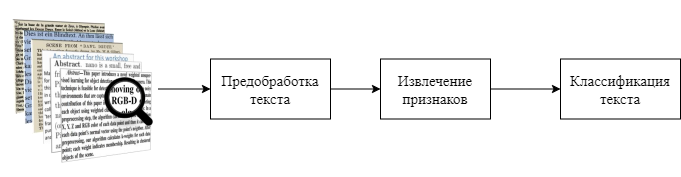
\includegraphics[,scale=0.7]{./img/system.png}
		\caption{Этапы процесса классификации текста.}  
		\label{img:system}
\end{figure}


Система классификации текстов содержит четыре различных уровня области применения, которые можно применять.
\begin{enumerate}
    \item Уровень документа. На этом уровне документа алгоритм получает соответствующие категории полного документа.
    \item Уровень абзаца. На этом уровне абзаца алгоритм получает соответствующие категории одного абзаца (части документа).
    \item Уровень предложения. На этом уровне предложения получают соответствующие категории одного предложения (части абзаца).
    \item Уровень подпредложения. На этом уровне подпредложения алгоритм получает соответствующие категории подвыражений внутри предложения.
\end{enumerate}